% Title: gl2ps_renderer figure
% Creator: GL2PS 1.4.0, (C) 1999-2017 C. Geuzaine
% For: Octave
% CreationDate: Tue May 11 13:35:41 2021
\setlength{\unitlength}{1pt}
\begin{picture}(0,0)
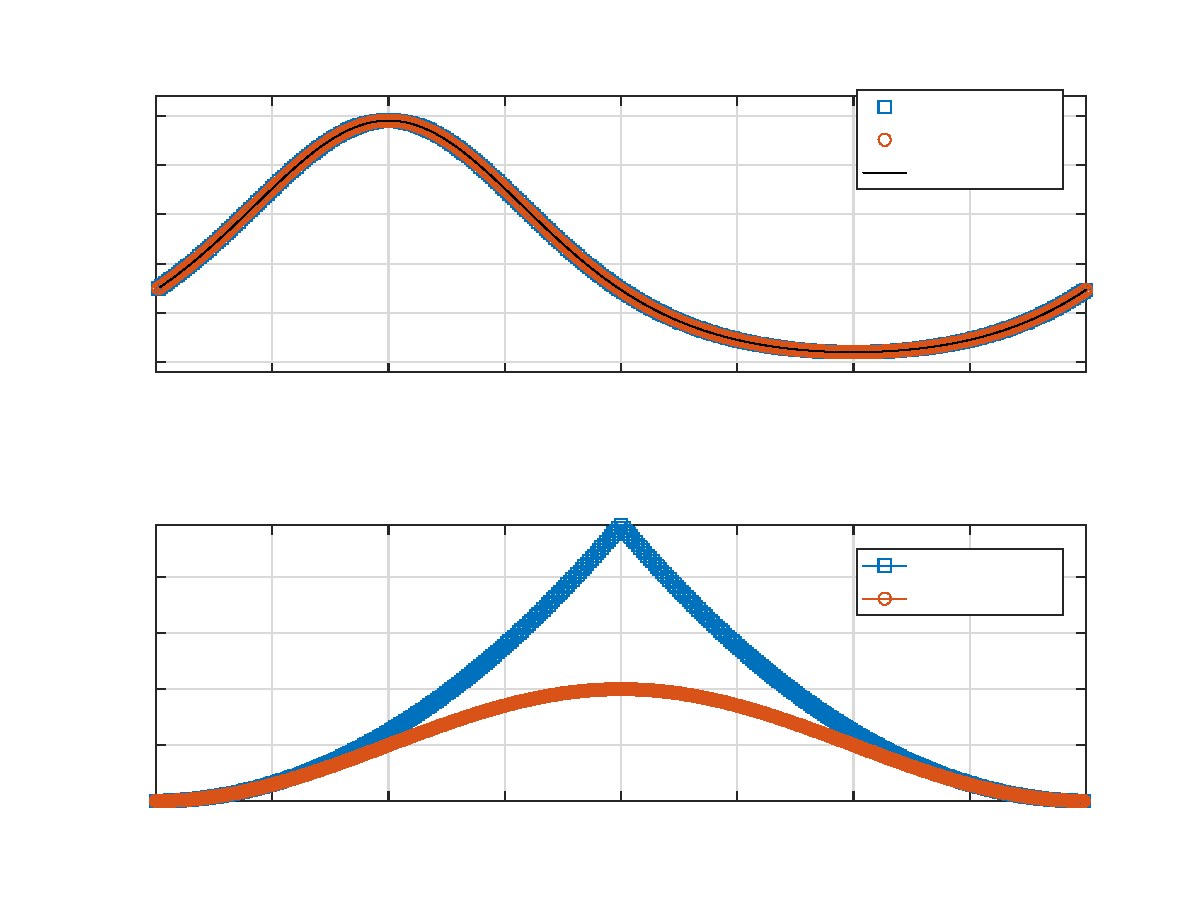
\includegraphics{figures/chap26/OUT/poisson384-inc}
\end{picture}%
\begin{picture}(576,432)(0,0)
\fontsize{10}{0}
\selectfont\put(74.88,245.874){\makebox(0,0)[t]{\textcolor[rgb]{0.15,0.15,0.15}{{0}}}}
\fontsize{10}{0}
\selectfont\put(130.68,245.874){\makebox(0,0)[t]{\textcolor[rgb]{0.15,0.15,0.15}{{0.25}}}}
\fontsize{10}{0}
\selectfont\put(186.48,245.874){\makebox(0,0)[t]{\textcolor[rgb]{0.15,0.15,0.15}{{0.5}}}}
\fontsize{10}{0}
\selectfont\put(242.28,245.874){\makebox(0,0)[t]{\textcolor[rgb]{0.15,0.15,0.15}{{0.75}}}}
\fontsize{10}{0}
\selectfont\put(298.08,245.874){\makebox(0,0)[t]{\textcolor[rgb]{0.15,0.15,0.15}{{1}}}}
\fontsize{10}{0}
\selectfont\put(353.88,245.874){\makebox(0,0)[t]{\textcolor[rgb]{0.15,0.15,0.15}{{1.25}}}}
\fontsize{10}{0}
\selectfont\put(409.68,245.874){\makebox(0,0)[t]{\textcolor[rgb]{0.15,0.15,0.15}{{1.5}}}}
\fontsize{10}{0}
\selectfont\put(465.48,245.874){\makebox(0,0)[t]{\textcolor[rgb]{0.15,0.15,0.15}{{1.75}}}}
\fontsize{10}{0}
\selectfont\put(521.28,245.874){\makebox(0,0)[t]{\textcolor[rgb]{0.15,0.15,0.15}{{2}}}}
\fontsize{10}{0}
\selectfont\put(69.8755,258.129){\makebox(0,0)[r]{\textcolor[rgb]{0.15,0.15,0.15}{{-1}}}}
\fontsize{10}{0}
\selectfont\put(69.8755,281.779){\makebox(0,0)[r]{\textcolor[rgb]{0.15,0.15,0.15}{{-0.5}}}}
\fontsize{10}{0}
\selectfont\put(69.8755,305.429){\makebox(0,0)[r]{\textcolor[rgb]{0.15,0.15,0.15}{{0}}}}
\fontsize{10}{0}
\selectfont\put(69.8755,329.079){\makebox(0,0)[r]{\textcolor[rgb]{0.15,0.15,0.15}{{0.5}}}}
\fontsize{10}{0}
\selectfont\put(69.8755,352.729){\makebox(0,0)[r]{\textcolor[rgb]{0.15,0.15,0.15}{{1}}}}
\fontsize{10}{0}
\selectfont\put(69.8755,376.379){\makebox(0,0)[r]{\textcolor[rgb]{0.15,0.15,0.15}{{1.5}}}}
\fontsize{11}{0}
\selectfont\put(298.08,395.839){\makebox(0,0)[b]{\textcolor[rgb]{0,0,0}{{Pseudo--Spectral and Finite Difference Approximations: $M = $ 384}}}}
\fontsize{11}{0}
\selectfont\put(46.8755,319.619){\rotatebox{90}{\makebox(0,0)[b]{\textcolor[rgb]{0.15,0.15,0.15}{{exact and approximate solutions}}}}}
\fontsize{11}{0}
\selectfont\put(298.08,232.874){\makebox(0,0)[t]{\textcolor[rgb]{0.15,0.15,0.15}{{$x$}}}}
\fontsize{12}{0}
\selectfont\put(353.88,325.532){\makebox(0,0)[l]{\textcolor[rgb]{0,0,0}{{max error ps = 1.166e-15}}}}
\fontsize{12}{0}
\selectfont\put(353.88,311.342){\makebox(0,0)[l]{\textcolor[rgb]{0,0,0}{{max error fd = 6.065e-05}}}}
\fontsize{9}{0}
\selectfont\put(438.176,380.725){\makebox(0,0)[l]{\textcolor[rgb]{0,0,0}{{pseudo--spectral}}}}
\fontsize{9}{0}
\selectfont\put(438.176,364.946){\makebox(0,0)[l]{\textcolor[rgb]{0,0,0}{{finite difference}}}}
\fontsize{9}{0}
\selectfont\put(438.176,349.168){\makebox(0,0)[l]{\textcolor[rgb]{0,0,0}{{exact}}}}
\fontsize{10}{0}
\selectfont\put(74.88,39.995){\makebox(0,0)[t]{\textcolor[rgb]{0.15,0.15,0.15}{{0}}}}
\fontsize{10}{0}
\selectfont\put(130.68,39.995){\makebox(0,0)[t]{\textcolor[rgb]{0.15,0.15,0.15}{{48}}}}
\fontsize{10}{0}
\selectfont\put(186.48,39.995){\makebox(0,0)[t]{\textcolor[rgb]{0.15,0.15,0.15}{{96}}}}
\fontsize{10}{0}
\selectfont\put(242.28,39.995){\makebox(0,0)[t]{\textcolor[rgb]{0.15,0.15,0.15}{{144}}}}
\fontsize{10}{0}
\selectfont\put(298.08,39.995){\makebox(0,0)[t]{\textcolor[rgb]{0.15,0.15,0.15}{{192}}}}
\fontsize{10}{0}
\selectfont\put(353.88,39.995){\makebox(0,0)[t]{\textcolor[rgb]{0.15,0.15,0.15}{{240}}}}
\fontsize{10}{0}
\selectfont\put(409.68,39.995){\makebox(0,0)[t]{\textcolor[rgb]{0.15,0.15,0.15}{{288}}}}
\fontsize{10}{0}
\selectfont\put(465.48,39.995){\makebox(0,0)[t]{\textcolor[rgb]{0.15,0.15,0.15}{{336}}}}
\fontsize{10}{0}
\selectfont\put(521.28,39.995){\makebox(0,0)[t]{\textcolor[rgb]{0.15,0.15,0.15}{{384}}}}
\fontsize{10}{0}
\selectfont\put(69.8755,47.52){\makebox(0,0)[r]{\textcolor[rgb]{0.15,0.15,0.15}{{0}}}}
\fontsize{10}{0}
\selectfont\put(69.8755,74.3579){\makebox(0,0)[r]{\textcolor[rgb]{0.15,0.15,0.15}{{2}}}}
\fontsize{10}{0}
\selectfont\put(69.8755,101.196){\makebox(0,0)[r]{\textcolor[rgb]{0.15,0.15,0.15}{{4}}}}
\fontsize{10}{0}
\selectfont\put(69.8755,128.034){\makebox(0,0)[r]{\textcolor[rgb]{0.15,0.15,0.15}{{6}}}}
\fontsize{10}{0}
\selectfont\put(69.8755,154.872){\makebox(0,0)[r]{\textcolor[rgb]{0.15,0.15,0.15}{{8}}}}
\fontsize{11}{0}
\selectfont\put(298.08,189.96){\makebox(0,0)[b]{\textcolor[rgb]{0,0,0}{{Normalized Eigenvalues of the Pseudo-Spectral and Finite Difference Operators}}}}
\fontsize{11}{0}
\selectfont\put(58.8755,113.74){\rotatebox{90}{\makebox(0,0)[b]{\textcolor[rgb]{0.15,0.15,0.15}{{normalized eigenvalues}}}}}
\fontsize{11}{0}
\selectfont\put(298.08,26.995){\makebox(0,0)[t]{\textcolor[rgb]{0.15,0.15,0.15}{{wave number, $k$}}}}
\fontsize{9}{0}
\selectfont\put(438.176,160.456){\makebox(0,0)[l]{\textcolor[rgb]{0,0,0}{{pseudo--spectral}}}}
\fontsize{9}{0}
\selectfont\put(438.176,144.678){\makebox(0,0)[l]{\textcolor[rgb]{0,0,0}{{finite difference}}}}
\end{picture}
